\begin{figure*}[h!]
    \begin{subfigure}{\linewidth}
        \caption{}
        \centering
        % include first image
        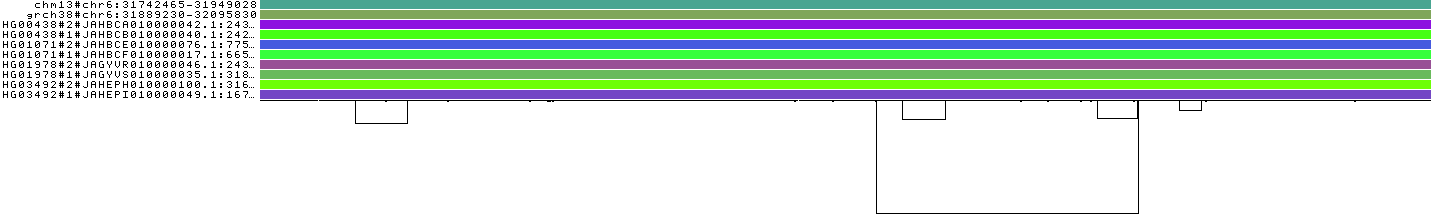
\includegraphics[width=1.0\linewidth, trim=0 +2cm 0 0]{fig/visualization_1D/chr6.pan.fa.a2fb268.e820cd3.9ea71d8.smooth.gfa.og.grch38_chr6_31889244-32095493.0.sorted}
        \label{fig:odgi_viz_default}
    \end{subfigure}
    \begin{subfigure}{\linewidth}
        \caption{}
        \centering
        % include second image
        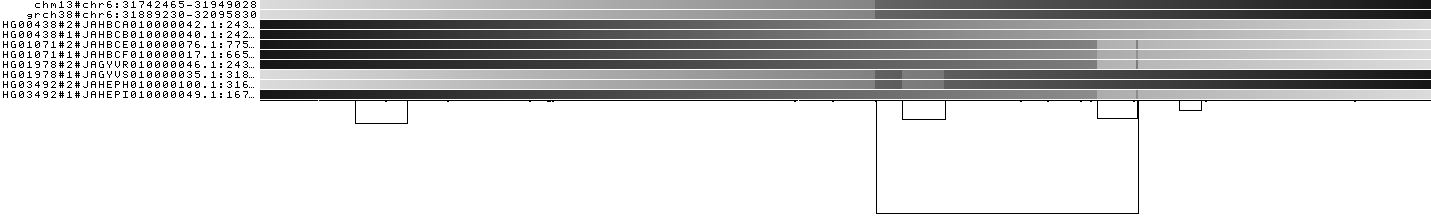
\includegraphics[width=1.0\linewidth, trim=0 +2cm 0 0]{fig/visualization_1D/chr6.pan.fa.a2fb268.e820cd3.9ea71d8.smooth.gfa.og.grch38_chr6_31889244-32095493.0.sorted.du}
        \label{fig:odgi_viz_color_by_path_pos}
    \end{subfigure}
    \begin{subfigure}{\linewidth}
        \caption{}
        \centering
        % include second image
        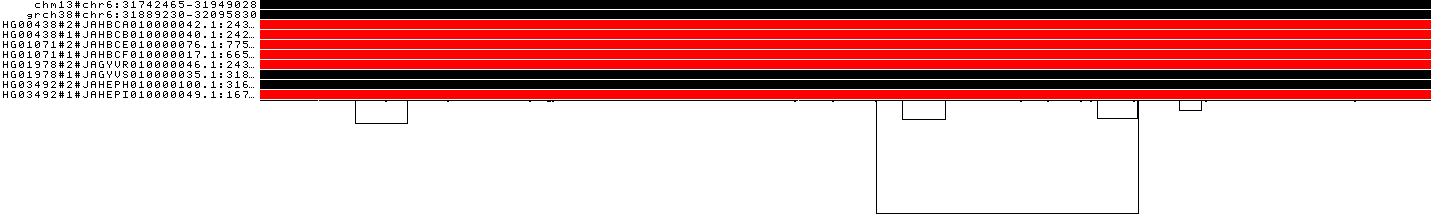
\includegraphics[width=\linewidth, trim=0 +2cm 0 0]{fig/visualization_1D/chr6.pan.fa.a2fb268.e820cd3.9ea71d8.smooth.gfa.og.grch38_chr6_31889244-32095493.0.sorted.z}
        \label{fig:odgi_viz_color_by_inversion_rate}
    \end{subfigure}
    \begin{subfigure}{1\linewidth}
        \caption{}
        \centering
        % include fourth image
        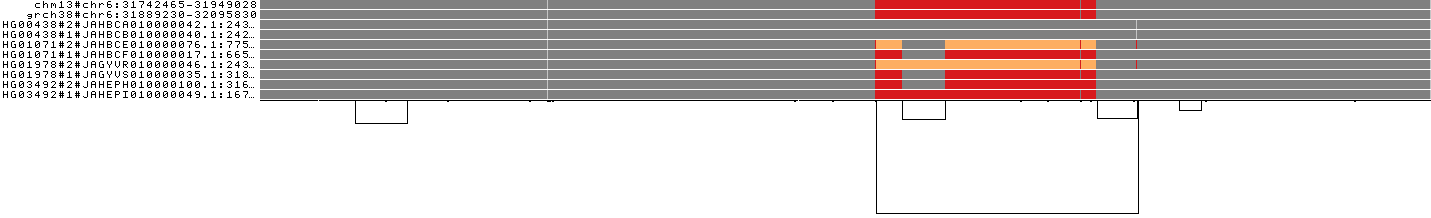
\includegraphics[width=\linewidth, trim=0 0 0 0]{fig/visualization_1D/chr6.pan.fa.a2fb268.e820cd3.9ea71d8.smooth.gfa.og.grch38_chr6_31889244-32095493.0.sorted.m}
        \label{fig:odgi_viz_color_by_path_depth}
    \end{subfigure}
    \caption{Visualizing the complement component 4 (C4) \textit{locus} from a human pangenome graph of 90 haplotypes: \textbf{(a)} standard mode: explain the bio stuff. \textbf{(b)} odgi viz's color by path position: explain the bio stuff XXX. \textbf{(c)} odgi viz's color by strandness: explain the bio stuff XXX. `textbf{(d)}  odgi viz's color by coverage: explain the bio stuff XXX.}
    \label{fig:odgi_viz}
\end{figure*}
